% Presentación: Transformada de Fourier y FFT
\documentclass[aspectratio=169]{beamer}
\usetheme{Madrid}
\usecolortheme{default}

\usepackage[spanish]{babel}
\usepackage{amsmath, amssymb}
\usepackage{graphicx}
\usepackage{hyperref}
\usepackage{tikz}

\newcommand{\imag}{\mathrm{j}}
 
\newcommand{\frt}[1]{\tilde{\text{f}}\left\{#1\right\}}


\newcommand{\frtn}[1]{\text{f}\left\{#1\right\}}
\newcommand{\frtP}[1]{\tilde{\text{f}}\left(#1\right)}

\newcommand{\frtnP}[1]{\text{f}\left(#1\right)}

% =========================
% INFORMACIÓN
% =========================
\title{Algoritmos Cuánticos}
\subtitle{Transformaciones integrales}
\author{Contreras Reyes Orlando \\García Barrera Iker  Emiliano\\ {\small Asesor: José Luis López González}}
\institute{Universidad Autónoma de Aguascalientes \\ Departamento de Sistemas Electrónicos}
\date{\today}

% ============================================================
\begin{document}
% ============================================================

% ------------------------------------------------------------
% PORTADA
% ------------------------------------------------------------
\begin{frame}
  \vspace{-0.3cm}
  \begin{columns}[c]
    \column{0.18\textwidth}
      \centering
      
\includegraphics[width=0.85\linewidth]{src/UAA.jpeg}
    \column{0.64\textwidth}
      \titlepage
    \column{0.18\textwidth}
      \centering
      
\includegraphics[width=0.95\linewidth]{src/IE.png}
  \end{columns}
\end{frame}



\begin{frame}{Contenido}
\tableofcontents
\end{frame}



\section{Transformaciones Integrales}
\subsection{¿Qué es una Transformación Integral?}
\begin{frame}{¿Qué es una Transformación Integral?}
\begin{block}{Definición}
Una transformación integral es una operación lineal que convierte una función \textbf{f}$(x)$ en otra función $\frt{s}$ a través de una integral definida.
\end{block}

\begin{equation*}
\tilde{\text{f}}(s) = \int_{x_a}^{x_b} K(s, x) \text{f}(x) dx
\end{equation*}

donde $K(s, x)$ es el \alert{núcleo de la transformación} que determina cómo se relacionan las funciones de entrada y salida. Además, $x_a$ y $x_b$ son los límites de integración de $x$, determinados por el dominio de definición de $f(x)$ y del núcleo $K(s,x)$.

\vspace{0.5cm}
\textbf{Característica clave:} Las transformaciones integrales son \textbf{lineales}.
\end{frame}


\subsection{Ejemplos de Transformaciones Integrales}
\begin{frame}{Ejemplos de Transformaciones Integrales}
\begin{itemize}
    \item \textbf{Laplace}: Ecuaciones diferenciales y sistemas en dominio temporal
    
    \item \textbf{Fourier}: Análisis de señales (dominio temporal $\rightarrow$ dominio de frecuencia)
    
    \item \textbf{Mellin}: Análisis asintótico y teoría de números
    
    \item \textbf{Z}: Procesamiento de señales discretas y análisis de sistemas discretos
\end{itemize}

\vspace{0.3cm}

\end{frame}

\section{Transformada de Fourier}
\subsection{Definición}
\begin{frame}{Transformada de Fourier - Definición}
\begin{block}{¿Qué es?}
Un modelo matemático que descompone una función en sus \alert{componentes de frecuencia}.
\end{block}


\begin{columns}[c]
\column{0.5\textwidth}
\textbf{Aplicaciones:}
\begin{itemize}
    \item Análisis de señales
    \item Procesamiento de imágenes
    \item Física
    \item Ingeniería
\end{itemize}
\begin{equation*}
\frtP{s} = \int_{-\infty}^{\infty} \frtnP{x}  e^{-(2\pi \imag) x} dx
\label{eq:furierrial}
\end{equation*}

\column{0.5\textwidth}
\begin{figure}
    \centering
    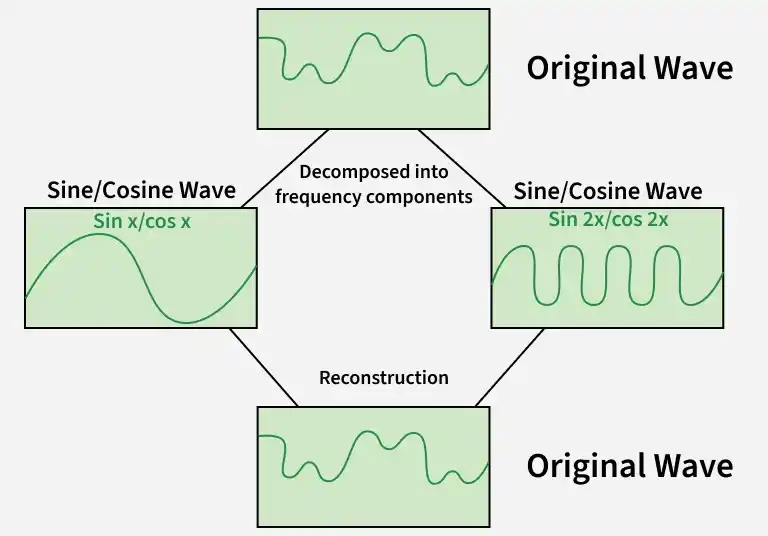
\includegraphics[width=0.8\textwidth]{src/Fourier.png}
    \caption{Transformada de Fourier}
\end{figure}
\end{columns}
\end{frame}


\subsection{Dominio Espacio-Tiempo}
\begin{frame}{Dominio Espacio-Tiempo}
\begin{columns}[c]
\column{0.5\textwidth}
\begin{block}{Ondas}
Una onda temporal puede representarse: 
Representación temporal
$$
f(t) = A\sin(\omega t + \phi), \quad \omega = 2\pi\nu = \dfrac{2\pi}{T}
$$
Representación espacial
$$
g(x) = B\sin(kx + \theta), \quad k = \dfrac{2\pi}{\lambda}
$$
\end{block}




\column{0.5\textwidth}
\begin{figure}
    \centering
    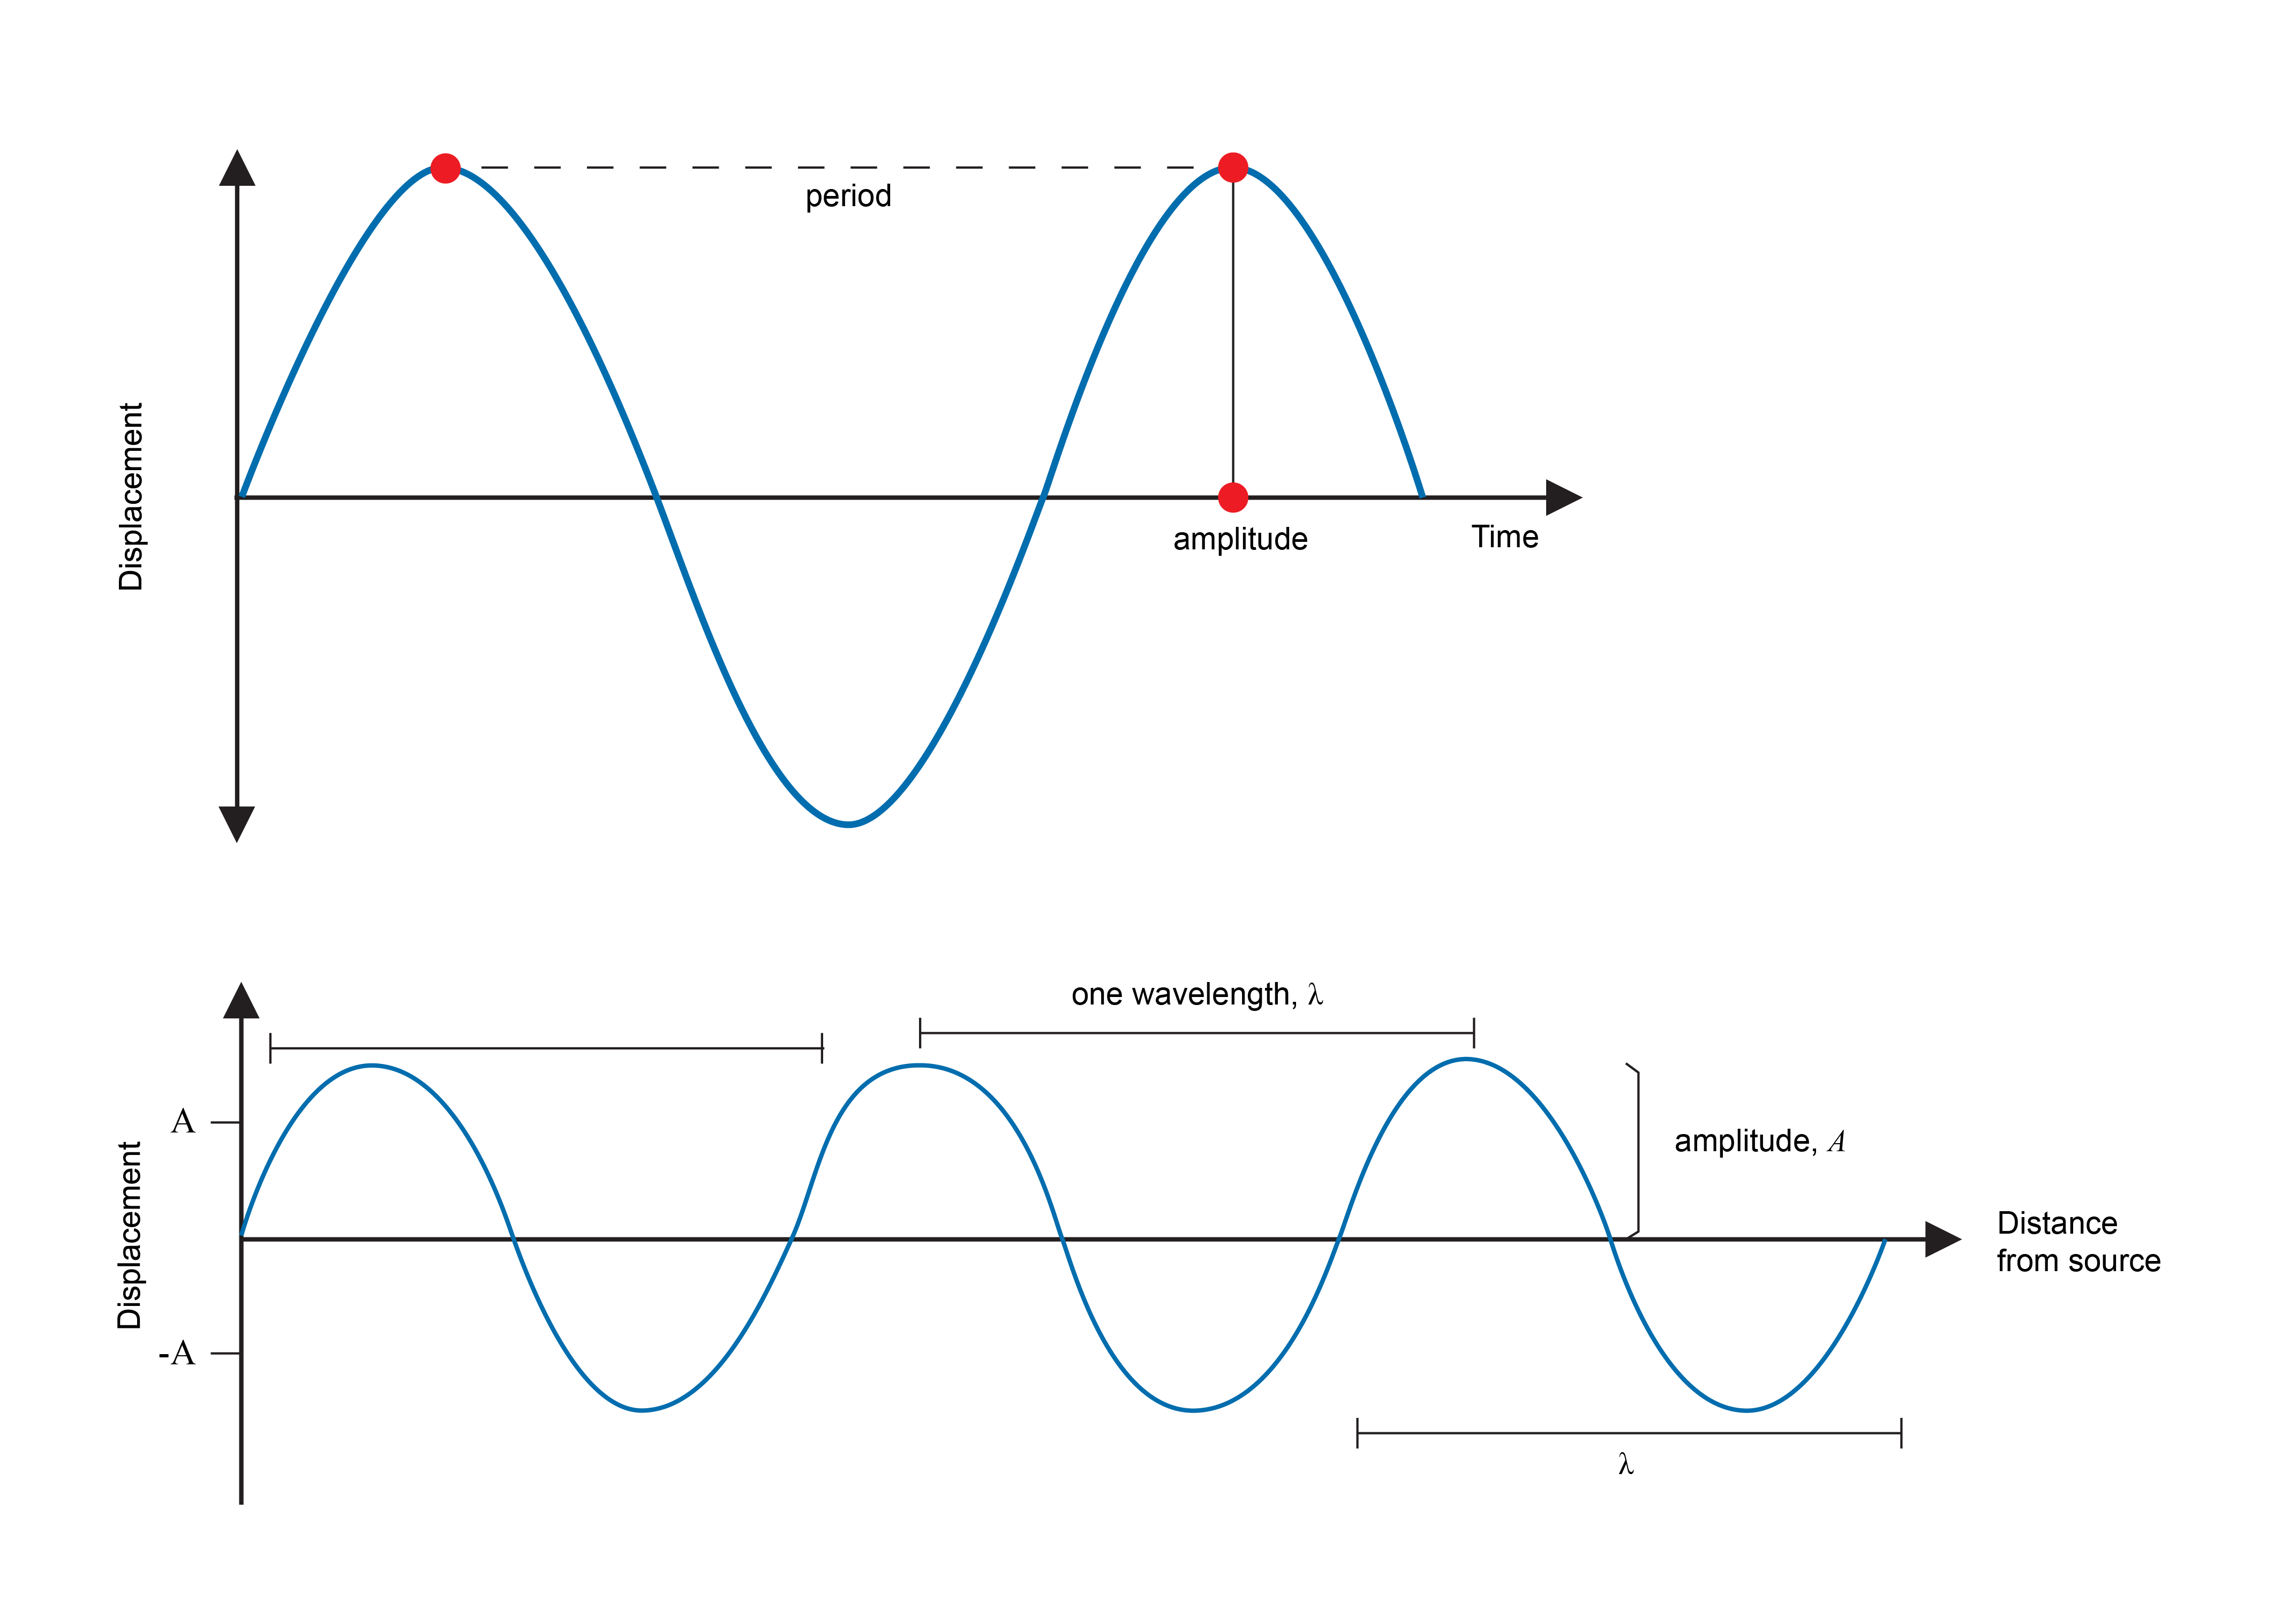
\includegraphics[width=0.9\textwidth]{src/waves.png}
    \caption{Onda temporal y espacial}
\end{figure}
\end{columns}
\end{frame}

\subsection{Representaciones}
\begin{frame}{Transformada de Fourier - Representaciones}
\begin{block}{¿Por qué trabajar en el tiempo?}
Se analiza en función del tiempo porque la transformada de Fourier parte de una señal temporal y la lleva al dominio de frecuencia.
\end{block}

\begin{columns}[c]
\column{0.35\textwidth}
\begin{block}{Transformada de Fourier}
Transformada directa
$$
\frtP{\nu} = \int_{-\infty}^{\infty} \frtnP{t} e^{-2\pi \imag \nu t} dt
$$
Transformada inversa
$$
\frtnP{t} = \int_{-\infty}^{\infty} \frtP{\nu} e^{2\pi \imag \nu t} d\nu
$$

\end{block}



\column{0.55\textwidth}
\begin{block}{Definiciones}
Tiempo ($t$): es la variable temporal y la variable independiente en la función original $f(t)$.
\newline\newline
Frecuencia ($\nu$): es la variable de frecuencia en el dominio transformado y la variable independiente en $\frtP{\nu}$.
\end{block}
\end{columns}
\end{frame}


\subsection{Convenciones}
\begin{frame}{Convenciones de la Transformada de Fourier}
La forma general utiliza dos constantes arbitrarias $a$ y $b$:

\begin{equation*}
\frtP{\nu} = \sqrt{\dfrac{|b|}{(2\pi)^{1-a}}}\int_{-\infty}^{\infty} \text{f}(t)\, e^{\imag b\nu t}\, dt
\quad
\frtnP{t} = \sqrt{\dfrac{|b|}{(2\pi)^{1+a}}}\int_{-\infty}^{\infty} \frtP{\nu}\, e^{-\imag b\nu t}\, d\nu
\end{equation*}

% \begin{table}
%   \centering
%   \small
%   \begin{tabular}{c|l}
%     \hline
%     \textbf{(a,b)} & \textbf{Uso típico} \\
%     \hline
%     (0,1) & Física moderna \\
%     (1,-1) & Matemáticas e ingeniería \\
%     (1,1) & Teoría de probabilidad \\
%     (-1,1) & Física clásica \\
%     (0,-2$\pi$) & Procesamiento de señales \\
%     \hline
%   \end{tabular}
% \end{table}
Para el caso de procesamiento de señales ($a=0 \quad b= -2 \pi$)


\begin{equation*}
\begin{aligned}
\frtP{\nu}
&= \sqrt{\dfrac{|-2\pi|}{(2\pi)^{1-0}}}\int_{-\infty}^{\infty} \frtnP{t}e^{j(-2\pi)\nu t}dt \\
&= \sqrt{1}\int_{-\infty}^{\infty} \frtnP{t}e^{j(-2\pi)\nu t}dt \\
&= \boxed{\int_{-\infty}^{\infty} \frtnP{t}e^{-j2\pi\nu t}dt}\\
\end{aligned}
\end{equation*}

\end{frame}


\begin{frame}{Transformada de Fourier }
\begin{block}{Derivación transformada de Fourier}
Retomando la definición anterior y considerando los puntos previos, definimos la transformada de Fourier de la siguiente manera:
$$
\frtP{\nu}=\int_{-\infty}^{\infty} \text{f}(t) e^{-\imag (2\pi \nu) t} dt
\Rightarrow \omega = 2\pi \nu
\Rightarrow \boxed{\frtP{\omega}=\int_{-\infty}^{\infty} \text{f}(t) e^{-\imag \omega t} dt}
$$
\end{block}


\begin{block}{Derivación transformada inversa de Fourier}
De la misma forma podemos obtener la transformada inversa de Fourier:

$$
\frtnP{t}= \int_{-\infty}^{\infty} \tilde{\text{f}}(\nu) e^{\imag (2\pi \nu) t} d\nu
\Rightarrow \omega = 2\pi \nu
\Rightarrow \boxed{\frtnP{t}=\dfrac{1}{2\pi}\int_{-\infty}^{\infty} \tilde{\text{f}}(\omega) e^{\imag \omega t} d\omega}
$$
\end{block}

\end{frame}


\subsection{Propiedades}
\begin{frame}{Propiedades de la Transformada de Fourier}

\begin{block}{Propiedades}
\textbf{1. Linealidad}
    $$\frt{a \text{f}_1 (t) + b \text{f}_2 (t)} = a \frt{\text{f}_1 (t)} + b \frt{\text{f}_2 (t)}$$
\textbf{2. Desplazamiento y 3. Escalamiento}
$$\frt{\text{f}(t - t_0)} = e^{-j \omega t_0} \frt{\text{f}(t)} \qquad  \frt{\text{f}(at)} = \frac{1}{|a|} \frt{\frac{\text{f}(t)}{a}}$$
\end{block}



\begin{figure}
    \centering
    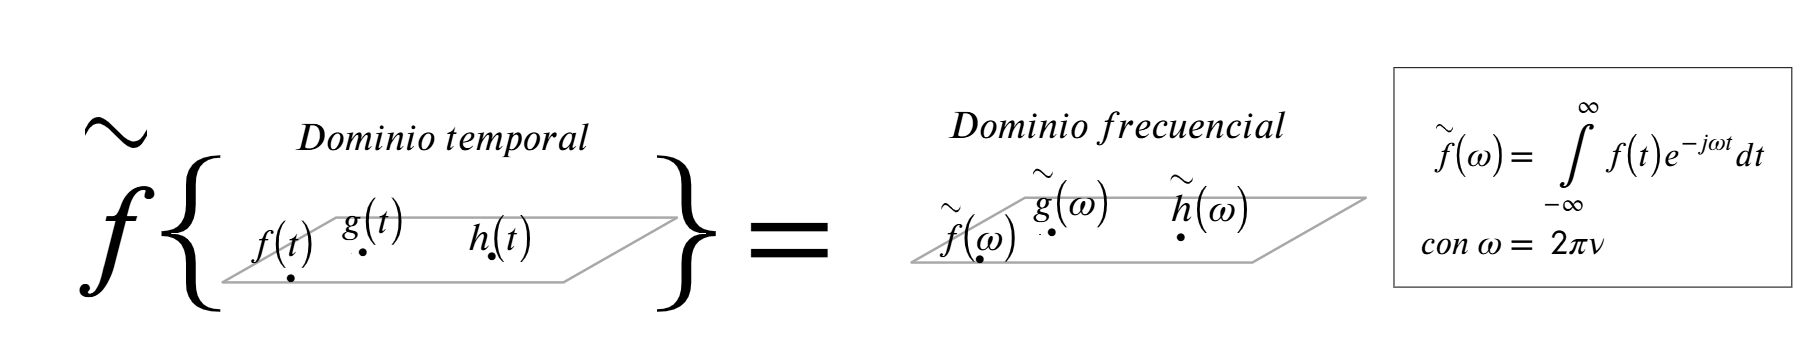
\includegraphics[width=0.8\linewidth]{src/Espasios.png}
    \caption{Dominio temporal y espacial}
\end{figure}



\end{frame}




% \begin{frame}{Propiedades de la Transformada de Fourier II}
% \begin{block}{4. Conjugación}
% $$\frt{f^*(x)} = \frt{f(x)}^*$$
% El conjugado de una funcion podria ser ejemplo
% $$f(x) = A e^{j \theta} \quad \Rightarrow \quad f^*(x) = A e^{-j \theta}$$
% \end{block}


% \begin{block}{5. Convolución}
% $$\frt{f(x) * g(x)} = \frt{f(x)} \cdot \frt{g(x)}$$
% \end{block}

% \vspace{0.3cm}
% \begin{alertblock}{Importante}
% La convolución en el dominio del tiempo se convierte en \alert{multiplicación} en el dominio de la frecuencia.
% \end{alertblock}
% \end{frame}

% \begin{frame}{Convolución - Definición}
% \begin{block}{¿Qué es la Convolución?}
% Integral que expresa la cantidad de solapamiento entre dos funciones a medida que una se desplaza sobre la otra.
% \end{block}

% \begin{equation*}
% (f * g)(t) = \int_{0}^{\infty} f(\tau) g(t - \tau) d\tau
% \end{equation*}

% \begin{figure}
%     \centering
%     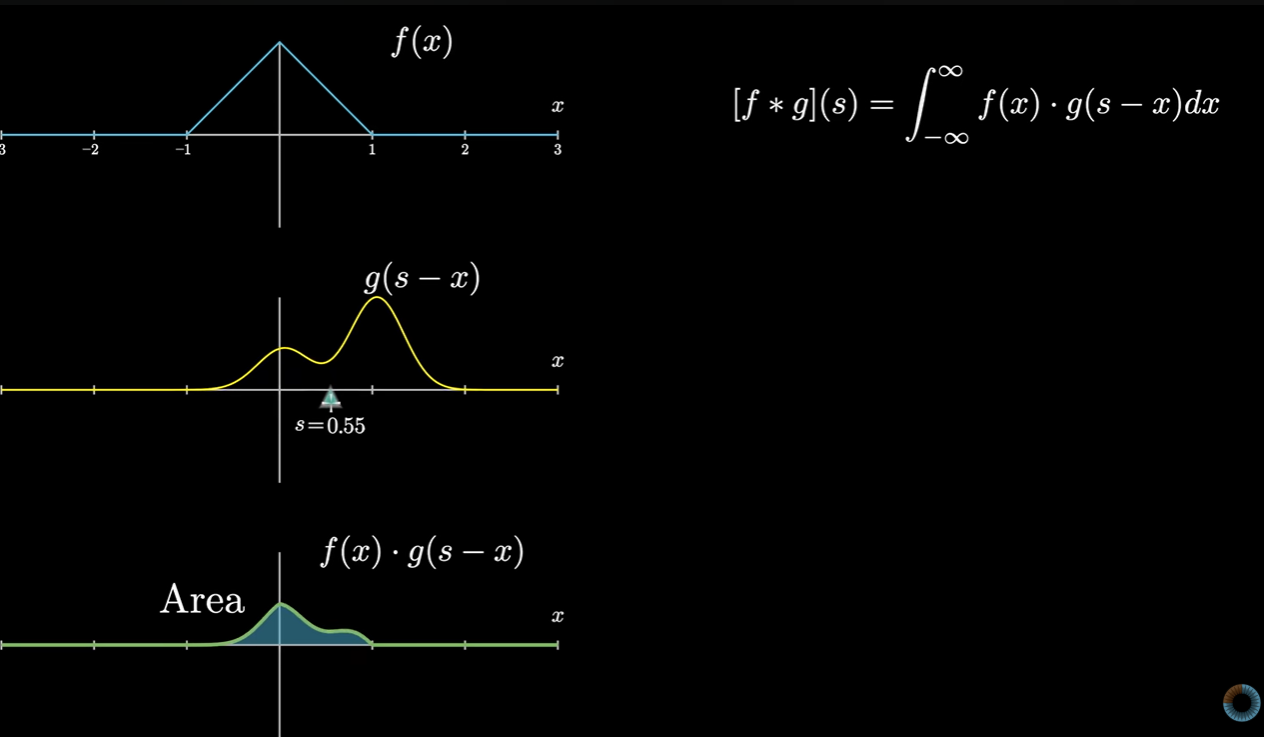
\includegraphics[width=0.4\textwidth]{src/Convolucion.png}
%     \caption{Visualización de la convolución}
% \end{figure}
% \end{frame}

\begin{frame}{Referencias Principales}
\begin{thebibliography}{99}
\bibitem{bracewell}
Bracewell, R. \textit{The Fourier Transform and Its Applications}, 3rd ed. McGraw-Hill, 1999.

\bibitem{wolfram-dft}
Wolfram MathWorld. \textit{Discrete Fourier Transform}. 
\url{https://mathworld.wolfram.com/DiscreteFourierTransform.html}

\bibitem{geeksforgeeks}
GeeksforGeeks. \textit{Fourier Transform}. 
\url{https://www.geeksforgeeks.org/maths/fourier-transform/}
\end{thebibliography}
\end{frame}


\end{document}